\chapter{Conceptos previos}


\section{Machine Learning}

Se entiende como el campo de las ciencias de computación que en vez de enfocarse en el diseño de algoritmos explícitos, optan por el estudio de técnicas de aprendizaje. Este enfoque tiene un gran éxito en tareas computacionales donde no es factible diseñar un algoritmo de forma explícita. \cite{Programming_Massively} \\
En vez de averiguar las distintas reglas a seguir para llegar a una solución, esta alternativa permite simplemente suministrar ejemplos de lo que debería pasar en distintas situaciones, y dejar que la máquina aprenda y extraiga ella misma sus propias conclusiones. De esta forma, el procedimiento en aprendizaje supervisado consiste en 'entrenar' con una muestra de N ejemplos, extraer información de ellos, y posteriormente poder evaluar de forma 'correcta' (bajo un margen de error controlado) otra muestra de M ejemplos, siendo M \textgreater N. \cite{Learning_From_Data} \\
Este enfoque ha contribuido en el avance de áreas como reconocimiento de voz, visión por ordenador, procesamiento de lenguaje natural, etc.

\section{Aprendizaje supervisado}

El aprendizaje supervisado se caracteriza por, a partir de una serie de datos de entrada X y sus etiquetas, entrenar un modelo con estos para que mediante un proceso iterativo este vaya aprendiendo de forma que al finalizar dicho entrenamiento el mismo modelo sea capaz de tomar mejores decisiones que antes de comenzarlo. \\
Suponiendo que nuestra muestra tiene N datos, tanto X como Y se unen para formar lo que se conoce como dataset D=\{($x_1, y_1$), ($x_2, y_2$), ..., ($x_N, y_N$)\}. Para que el aprendizaje sea posible, debe existir una función F: X $\rightarrow$ Y tal que $y_i$ = F($x_i$) para i$\in$\{1...N\}. De esta forma, en función del dataset D, el modelo tratará de encontrar una función G que aproxime F para dicho conjunto. Además, se suelen aplicar técnicas que permitan una mejor generalización del modelo, expandiendo las capacidades del mismo y permitiendo que su conocimiento pueda ser útil incluso fuera de la muestra de datos inicial. \cite{Learning_From_Data}

\section{División de datos en entrenamiento y test}

Suponiendo que a partir de unos datos de entrada y un modelo, logremos que este los emplee para aprender, normalmente el objetivo final es emplear dicho modelo fuera de esa muestra inicial. \\
Por ejemplo, en el caso de aprender a montar en bici lo que se suele querer es aprender a montar en cualquier bici, no aprender a usar una bici y cada vez que se quiera cambiar de vehículo tener que volver a empezar dicho aprendizaje. \\
En el caso de los modelos de aprendizaje automático, un ejemplo simple puede ser distinguir gatos de perros. Si se entrena un modelo con 200 imágenes, suele ser común que su desarrollador quiera emplear dicho modelo entrenado para distinguir gatos de perros con imágenes que este no vio nunca antes. \\
Es decir, aunque se entrene un modelo con una muestra de N imágenes, es importante saber que en la mayoría de los casos lo que se busca no es un buen rendimiento exclusivamente en la muestra con que se entrenó, sino también en aquellas muestras en las que no se entrenó. \\
Para visualizar la generalización del modelo, el conjunto de datos D se suele dividir en 2 subconjuntos, (entrenamiento y test) de forma que se pueda estimar si realmente 'aprende' o solo memoriza.\\
Una vez realizada la división, se entrena el modelo con los datos del conjunto de entrenamiento. Cuando se termina el entrenamiento, se accede al conjunto test y se visualiza el rendimiento del modelo sobre el mismo. Como los datos de test no se emplearon en ningún momento, aportan una estimación sobre la generalización del modelo fuera de la muestra con la que se entrenó. 

\section{Redes Neuronales Totalmente Conectadas}

Antes de analizar las redes neuronales convolucionales (CNNs), tiene sentido empezar por las redes neuronales `clásicas' o totalmente conectadas. \\
Una red neuronal se trata de un programa o modelo de machine learning que toma decisiones de forma similar al cerebro humano, empleando para ello procesos que imitan a los de las neuronas biológicas \cite{NN_intro}. \\
Estas cuentan con una serie de neuronas artificiales organizadas por capas, y se caracterizan por tener una capa de entrada, una o varias capas ocultas y una capa de salida.

\subsection{Neurona}

\begin{figure}[H]
	\centering
	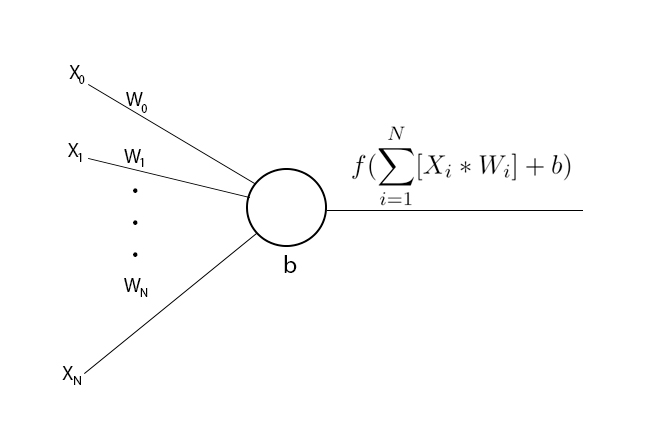
\includegraphics[scale=0.35]{imagenes/neurona.jpg}  
	\caption{Imagen de una neurona}
	\label{fig:neurona}
\end{figure}

Una neurona parte de una serie de datos de entrada X=\{$x_1$, $x_2$, ..., $x_N$\} tal que cada $x_i$$\in${X} se encuentra asociado a un peso $w_i\in{W}$. \\
En la Figura \ref{fig:neurona} se muestra como esta los emplea para realizar una suma ponderada y posteriormente añadir un sesgo b, además de aplicar una función de activación f sobre el resultado obtenido. 

\subsection{Estructura por capas}

\begin{figure}[H]
	\centering
	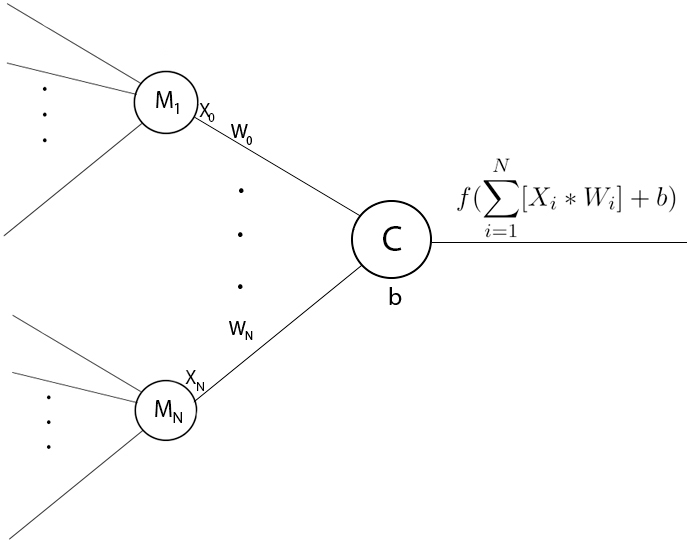
\includegraphics[scale=0.35]{imagenes/capa_neuronas.jpg}  
	\caption{Imagen de una capa de neuronas}
	\label{fig:capa_neuronas}
\end{figure}

Las neuronas se suelen agrupas por capas, de tal forma que la salida de una compone la entrada de la siguiente, formando así modelos más sofisticados (Figura \ref{fig:capa_neuronas}). \\
En este proyecto se desarrollarán redes neuronales para tareas de clasificación multiclase. Para clasificar N clases distintas, la capa de salida tendrá N neuronas. De esta forma, nuestra red totalmente conectada tendrá una capa de entrada (para recibir los datos de entrenamiento), una capa de salida, y las capas intermedias entre ellas recibirán el nombre de capas ocultas. 

\subsection{Funciones de activación}

Una función de activación en el contexto de las redes neuronales es una función matemática aplicada a la salida de una neurona. Su objetivo consiste en introducir no linealidad en el modelo, permitiendo que la red aprenda e identifique patrones complejos en los datos. Sin no linealidad, una red neuronal se comportaría esencialmente como un modelo de regresión lineal, independientemente del número de capas que tenga \cite{funcion_activacion_definicion}.

\subsubsection{ReLU}

\begin{gather}
	ReLU(x) = max(0, x)
\end{gather}

\begin{figure}[H]
	\centering
	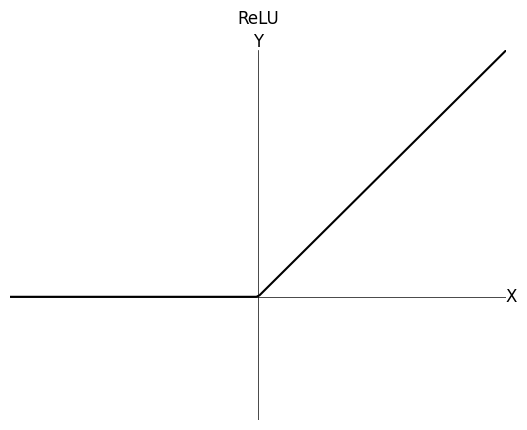
\includegraphics[scale=0.45]{imagenes/ReLU.jpg}  
	\caption{Imagen de la función de activación ReLU}
	\label{fig:ReLU}
\end{figure}

A cambio de un bajo coste computacional, la función de activación ReLU (Figura \ref{fig:ReLU}) aporta no linealidad a la neurona, permitiendo a esta aprender funciones de mayor complejidad. \\
Como su gradiente es 0 o 1 (0 para valores negativos, 1 para valores positivos), evita una reducción excesiva del mismo para valores positivos, mitigando así el problema del desvanecimiento del gradiente, caracterizado por la presencia de gradientes muy pequeños en retropropagación (se analizará con detalle en secciones posteriores) y provocar un aprendizaje lento \cite{ReLU}. \\
Además, tal y como sugieren los expertos, se empleará ReLU como función de activación en las capas intermedias de los modelos a implementar \cite{importancia_ReLU} \cite{importancia_ReLU_2}. 

\subsubsection{Sigmoide}

\begin{gather}
	sigmoide(x) = \frac{1}{1+e^{-x}}
\end{gather}

\begin{figure}[H]
	\centering
	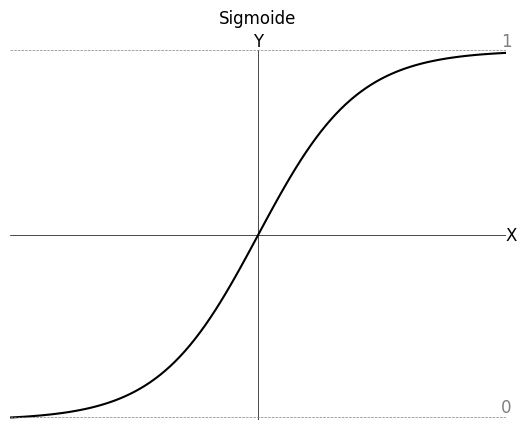
\includegraphics[scale=0.45]{imagenes/sigmoide.jpg}  
	\caption{Imagen de la función de activación Sigmoide}
	\label{fig:Sigmoide}
\end{figure}

La función de activación Sigmoide se trata de una función interesante en el ámbito de la clasificación binaria, pues se caracteriza por transformar un valor de entrada en una salida comprendida en el rango [0-1] , tal y como se muestra en la Figura \ref{fig:Sigmoide}. \\
Aunque sea monótona creciente y diferenciable en todos los puntos, tiende a saturarse con valores extremos (positivos o negativos). Por tanto, su aplicación dependerá del caso concreto a tratar. \cite{Sigmoide}

\subsection{Capa SoftMax}

\begin{figure}[H]
	\centering
	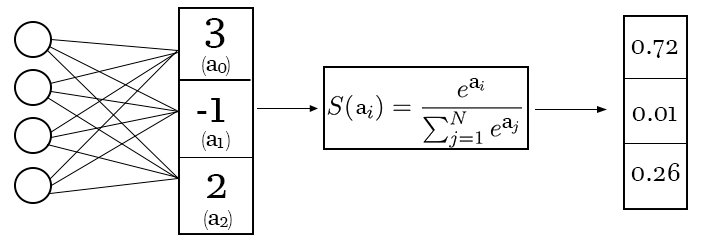
\includegraphics[scale=0.35]{imagenes/softmax.jpg}  
	\caption{Imagen de la función de activación SoftMax}
	\label{fig:SoftMax}
\end{figure}

La función SoftMax se suele emplear en la capa de salida de la red. Se caracteriza por, para n entradas, producir n salidas con valores en el rango [0-1] que mantienen la proporción de entrada y cuya suma es 1. Por tanto, cada salida i se puede interpretar como la probabilidad de pertenencia a la clase i, siendo especialmente útil en clasificación multiclase. \cite{SoftMax_MLM} \\
De esta forma, en la Figura \ref{fig:SoftMax} se muestra un ejemplo de clasificación multiclase con 3 clases distintas. \\
Para una entrada dada, el modelo estima que esta pertenece a la clase 0, pues este según este, dicha entrada presenta un 0.72\% de probabilidades de pertenecer a la clase 0, un 0.01\% a la clase 1, y un 0.26\% a la clase 2.


\subsection{Tipos de codificaciones de etiquetas}

En el campo de machine learning existen varios tipos de codificaciones. Así, para codificar 3 clases distintas se podrían codificar o bien mediante \{1, 2, 3\}, o mediante \{100, 010, 001\} (codificación one-hot), por ejemplo. En este proyecto se empleará la codificación one-hot por simplicidad y coincidir con la gran mayoría de bibliografía online.

\subsection{Función de error o pérdida}

En modelos de aprendizaje automático se suele emplear una función de optimización iterativa como descenso del gradiente (se muestra en el siguiente apartado) para, a partir de una función de error y unos datos de entrada, estimar el error del modelo sobre los mismos, y poder emplear dicha información para ir reduciendo el error iteración a iteración y así ir aprendiendo. 

\subsubsection{Entropía Cruzada}

\begin{gather}
	E(y, \hat{y}) = - \sum_{i=1}^{H}  [y_i * log( \hat{y}_i)]
	\label{fig:loss_func_softmax}
\end{gather}

En los modelos a desarrollar en este proyecto se empleará Entropía Cruzada como función de error por ser una métrica empleada en aprendizaje automático para medir qué tan bien se desempeña un modelo de clasificación. La pérdida o error se mide como un valor en el rango [0-1], siendo 0 un modelo perfecto y 1 otro totalmente erróneo. \cite{Cross_entropy}

En la fórmula \ref{fig:loss_func_softmax} se muestra el cálculo de la misma, donde H es el número de clases al que puede pertenecer cada dato de entrada $x_i \in X$, $y_i$ representa la etiqueta real de la entrada $x_i$ empleada, y $\hat{y}_i$ representa la etiqueta que el modelo predijo dicha entrada $x_i$.  \\

\subsubsection{Importancia de la función de error en el aprendizaje}

Para visualizar el papel de la función de error en el aprendizaje de un modelo, supondremos que los datos actuales cuentan con H=3 clases tal que para un $x_i \in X$ dado y empleando la codificación One-Hot para las etiquetas se tiene que $y_i = [0, 0, 1]$. 

\begin{gather}
	E(y, \hat{y}) = - \sum_{i=1}^{H}  [y_i * log( \hat{y}_i)] = 0 + 0 + log(0.1) = -log(0.1) = 2.3
	\label{ejemplo_1}
\end{gather}

Como la configuración inicial del modelo es desconocida, se supone que sus predicciones iniciales para $x_i$ son $\hat{y_i} = [ 0.6, 0.3, 0.1]$. En este caso, $x_i$ pertenece a la clase 3 pero el modelo predice que pertenece a la clase 1, pues 0.6 se interpreta como la probabilidad de pertenecer a la clase 1 y es la probabilidad más grande de todo $\hat{y_i}$.\\
Por tanto, su función de error indicaría que el error obtenido viene dado por la fórmula \ref{ejemplo_1}.

\begin{gather}
	E(y, \hat{y}) = - \sum_{i=1}^{H}  [y_i * log( \hat{y}_i)] = 0 + 0 + log(0.6) = -log(0.6) = 0.5
	\label{ejemplo_2}
\end{gather}

Tras entrenar el modelo durante varias iteraciones, $y_i$ permanece constante, pero $\hat{y_i}$ se modifica a $\hat{y_i} = [0.1, 0.3, 0.6]$, de forma que el nuevo error obtenido vendría dado por la fórmula \ref{ejemplo_2}, y ahora el modelo realizaría una predicción correcta sobre la clase de $x_i$, aunque todavía le quedaría margen de mejora pues el error es de 0.5 y este se puede minimizar. \\
De esta forma, se visualiza como a lo largo del entrenamiento de un modelo este se centra en reducir el error obtenido, y como consecuencia de ello va modificando sus predicciones de tal forma que se vayan ajustando a lo especificado por sus datos de entrada y etiquetas asociadas.


% https://medium.com/mlearning-ai/understanding-loss-functions-for-classification-81c19ee72c2a

\subsection{Descenso del gradiente}

\begin{figure}[H]
	\centering
	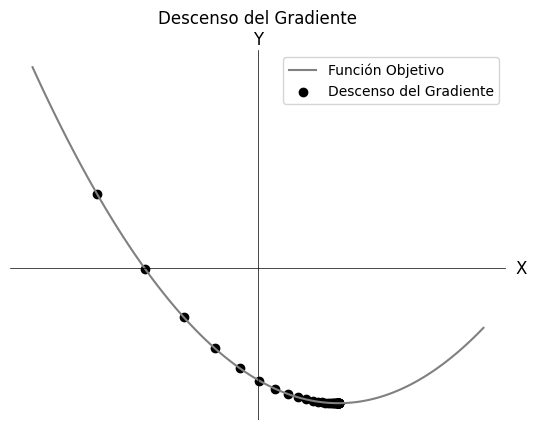
\includegraphics[scale=0.4]{imagenes/sgd.jpg}  
	\caption{Ejemplo de funcionamiento del descenso del gradiente}
	\label{fig:SGD}
\end{figure}

Tal y como se comentaba anteriormente, se trata de un método de optimización iterativo que busca el mínimo en una función diferenciable. En la figura \ref{fig:SGD} se muestra un ejemplo del mismo, donde la función objetivo hace referencia a la función de pérdida, y cada punto sobre ella representa una iteración del algoritmo, indicando como el error del modelo sobre la muestra se va reduciendo con cada iteración. \\
Su nombre viene del término 'gradiente', siendo este una generalización multivariable de la derivada y denominado por el símbolo $\nabla$. Para una función f y un punto p, este indica la dirección del máximo incremento en la misma. El descenso del gradiente usa esta información para, una vez obtenido el gradiente, desplazarse en dirección contraria, es decir, en dirección del mínimo. Además, la distancia que se recorre en cada iteración viene dada por un hiperparámetro denominado ``learning rate'' o $\alpha$ \cite{SGD_1} \cite{Gradiente} \cite{SGD_2}. \\
A diferencia de los parámetros de un modelo (pesos y sesgos), sus hiperparámetros son establecidos por el usuario y no se ``aprenden'' durante el entrenamiento del modelo.


\subsection{Inicialización de pesos}
Tal y como sugieren los expertos, se inicializarán los pesos mediante la ``inicialización He'' o ``inicialización Kaiming He''. Esta consiste en, para un peso $w$, inicializarlo según una distribución gaussiana con una media de 0.0 y una desviación típica de $\sqrt{\frac{2}{N\_in}}$, siendo $N\_in$ el número de neuronas en la capa de entrada
\cite{ini_He} \cite{ini_He_2} \cite{ini_He_code} \cite{importancia_ReLU} \cite{importancia_ReLU_2}.

\subsection{Inicialización de sesgos}

De la misma forma, se vuelve a seguir la bibliografía, indicando esta vez una inicialización de sesgos a 0.0 \cite{ini_bias} \cite{ini_bias_2}.

\subsubsection{Actualización de parámetros}
El procedimiento para entrenar una red neuronal consiste en, para una entrada $x_i$ y una etiqueta asociada $y_i$, emplear $x_i$ para realizar una predicción $\hat{y}_i$ (Propagación hacia delante de $x_i$ por la red) que posteriormente se podrá comparar con $y_i$ mediante una función de error H(x) y obtener una medida de lo buena o mala que fue la misma. Una vez obtenido dicho ``error'', se aplica el algoritmo del descenso del gradiente para obtener el gradiente de la pérdida respecto a cada parámetro de la red (Retropropagación) \cite{Cross_entropy}. \\

\begin{gather}
	W_{t+1} = W_{t} - \alpha * \frac{\partial H(x)}{\partial W_{t}} 
	\label{act_pesos}
\end{gather}

\begin{gather}
	b_{t+1} = b_{t} - \alpha * \frac{\partial H(x)}{\partial b_{t}}
	\label{act_bias}
\end{gather}


Así, se actualizarán los parámetros de la red neuronal (pesos y sesgos) según las fórmulas \ref{act_pesos} y \ref{act_bias}. En ellas, $W_t$ y $b_t$ indican los valores del peso W y bias b en el instante o iteración t, de la misma forma que $W_{t+1}$ y $b_{t+1}$ representan los valores de los mismos en el instante t+1 \cite{SGD_act_params}. \\
Es decir, dada una iteración t y unos datos de entrada X, primero se realiza la propagación hacia delante de los mismos a lo largo del modelo para obtener  $\hat{Y}$ o la predicción de los mismos. Una vez obtenida $\hat{Y}$, se emplea la función de error para obtener el error del modelo sobre los datos de entrada y, con ello, se realiza la retroprogacación del gradiente de la pérdida o error a lo largo del modelo, de forma que cada parámetro del mismo obtenga el gradiente de la pérdida respecto a él. Una vez cada parámetro tiene su gradiente respecto a la pérdida, lo emplea junto con $\alpha$ para actualizar su valor, dirigiéndose en dirección contraria al gradiente en una magnitud igual a $\alpha$ y poder reducir el posterior error en la iteración t+1. Los parámetros se actualizan una vez por iteración, tras realizar la retropropagación.

\subsubsection{Descenso del gradiente estocástico}

\begin{algorithm}[H]
	\caption{Descenso del gradiente estocástico \cite{SGD_3}} 
	\begin{algorithmic}
		\For{época $p\in\{0, ..., P-1\}$}
			\State Desordenar datos de entrenamiento.
			
			\For{$minibatch \in [m_{inicio}, ..., m_{fin}]$}
				\State Obtener datos del minibatch.
				\State Realizar propagación hacia delante.
				\State Obtener error mediante función de error.
				\State Realizar retropropagación y obtener gradiente de la pérdida   
				\State       respecto a cada parámetro del modelo.
				\State Actualizar parámetros.
			\EndFor
		\EndFor
	\end{algorithmic}
\end{algorithm}

Es una variante que sustituye el gradiente real por una estimación del mismo, logrando reducir la carga computacional y tiempo de entrenamiento a cambio de una menor tasa de convergencia \cite{sgd_stocastico} \cite{sgd_stocastico_1}. \\
Se caracteriza por, en cada época, dividir el conjunto de entrenamiento en varios subconjuntos aleatorios y disjuntos entre ellos (minibatch). \\
Para cada minibatch, se realiza la propagación hacia delante, cálculo de error, retropropagación y actualización de parámetros en ese orden. Se define como época la iteración del modelo por todos los minibatches \cite{sgd_stocastico}. \\

\section{Redes Neuronales Convolucionales}

\subsection{Introducción a CNNs}

Las redes neuronales convolucionales (CNN, Convolutional Neural Network) se caracterizan por trabajar con volúmenes de datos 3D. En este proyecto, se emplearán imágenes RGB como entrada para cada CNN. Por tanto, por simplificar la nomenclatura, cada capa 2D de un volumen 3D se denominará como imagen, pues una imagen RGB se trata de 3 imágenes 2D, una por color. Además, la entrada de cada capa se define como X o X(C*H*W) y en ambos casos cuenta con unas dimensiones de C*H*W, siendo C el número de canales de profundidad, H el número de filas y W el número de columnas de dicho volumen 3D. De la misma forma, se define el volumen de salida como Y($M*H_{out}*W_{out}$). En cuanto a los pesos de la capa convolucional, cada filtro o kernel se denominará mediante un símbolo/s diferente/s (K,K1, G, etc), pues cada uno puede presentar unas dimensiones diferentes. Aun así, se podrá definir a un filtro de pesos como K1(K*K), indicando que posee K filas y columnas. Además, también se trata de una estructura con 3 dimensiones. Sin embargo, no se requiere especificar el número de canales de profundidad de un kernel de pesos pues siempre será C (depende de X). De la misma forma, el número de filtros a aplicar sobre X recibe el nombre de M, y el tamaño de Y depende de este, pues tal y como se verá posteriormente, cada filtro genera una canal de profundidad distinto de la salida Y. 

\subsection{Capa convolucional}

\subsubsection{Componentes}


\begin{figure}[H]
	\centering
	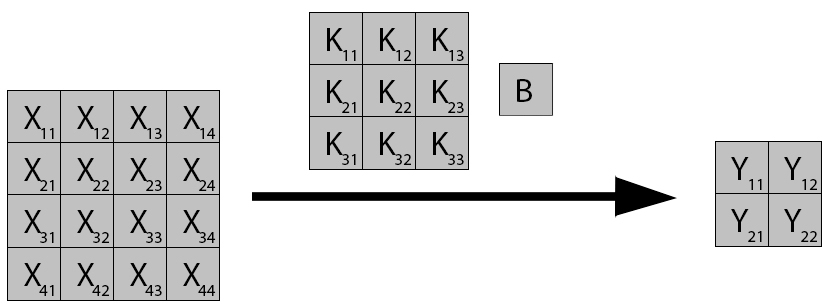
\includegraphics[scale=0.35]{imagenes/conv_nombres.jpg}  
	\caption{Componentes en una capa convolucional}
	\label{fig:Componentes_convolucion}
\end{figure}

Una capa convolucional parte de un volumen de entrada X, un kernel de filtros K, un sesgo B y una función de activación para, mediante una convolución, obtener un volumen de salida Y \cite{capa_convolucional} \cite{capa_convolucional_Stanford}.

\subsubsection{Propagación hacia delante}

\begin{figure}[H]
	\centering
	\begin{subfigure}{.5\textwidth}
		\hspace{-10mm}
		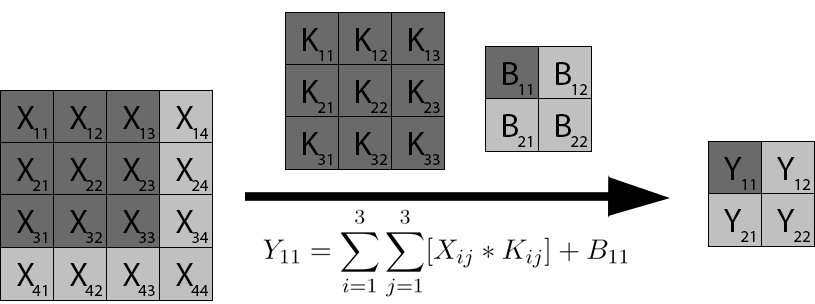
\includegraphics[width=1.2\linewidth]{imagenes/conv_1.jpg}  
		\caption{Cálculo $Y_{11}$}
	\end{subfigure}%
	\begin{subfigure}{.5\textwidth}
		\hspace{10mm}
		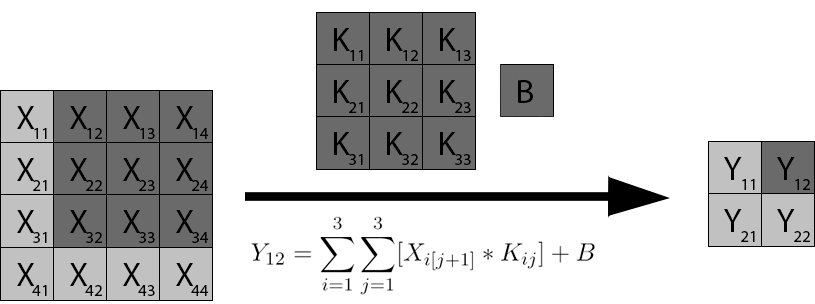
\includegraphics[width=1.2\linewidth]{imagenes/conv_2.jpg}  
		\caption{Cálculo $Y_{12}$}
	\end{subfigure}
	
	\vspace{5mm}
	\begin{subfigure}{.5\textwidth}
		\hspace{-10mm}
		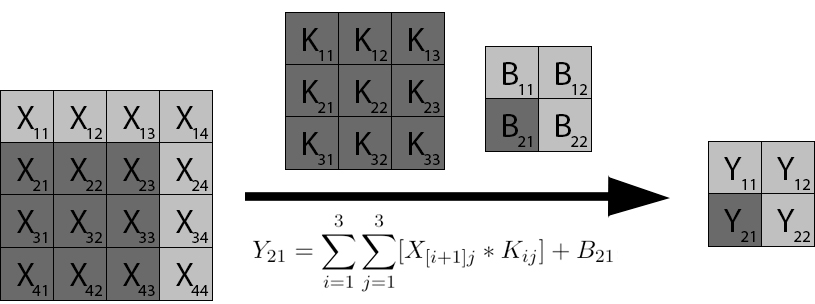
\includegraphics[width=1.2\linewidth]{imagenes/conv_3.jpg}  
		\caption{Cálculo $Y_{21}$}
	\end{subfigure}%
	\begin{subfigure}{.5\textwidth}
		\hspace{10mm}
		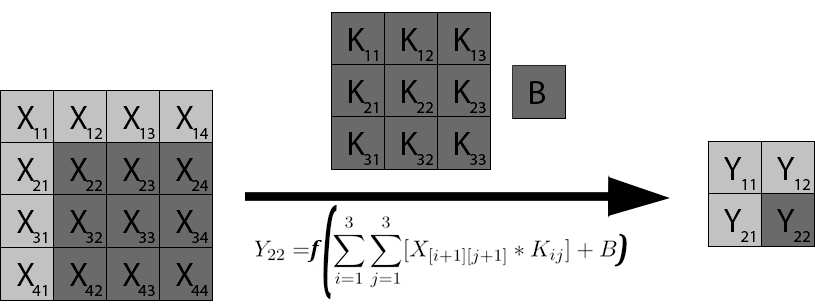
\includegraphics[width=1.2\linewidth]{imagenes/conv_4.jpg}  
		\caption{Cálculo $Y_{22}$}
	\end{subfigure}
	\caption{Propagación hacia delante en una capa convolucional}
	\label{fig:forward_prop_convolucional}
\end{figure}

Una convolución entre 2 volúmenes de datos X y K, consiste en ``deslizar K sobre X'' tal y como se muestra en la Figura \ref{fig:forward_prop_convolucional}. 
De esta forma, en cada ``paso'' se recorren ambos volúmenes, multiplicando los elementos de X y K 
que se encuentren en la misma posición. Posteriormente, se suma cada resultado obtenido, además de un sesgo B y finalmente aplicar una función de activación \cite{capa_convolucional}. \\
En la Figura \ref{fig:forward_prop_convolucional} se emplea un volumen X con un solo canal de profundidad. Sin embargo, este no es el caso común. Por tanto, se denotará como $X^{c}_{ij}$ al elemento de X que se encuentre en la posición (i,j) del canal de profundidad c \cite{capa_convolucional_Stanford}.

\subsubsection{Propagación hacia delante, canales de profundidad}

\begin{figure}[H]
	\centering
	\begin{subfigure}{.5\textwidth}
		\hspace{-10mm}
		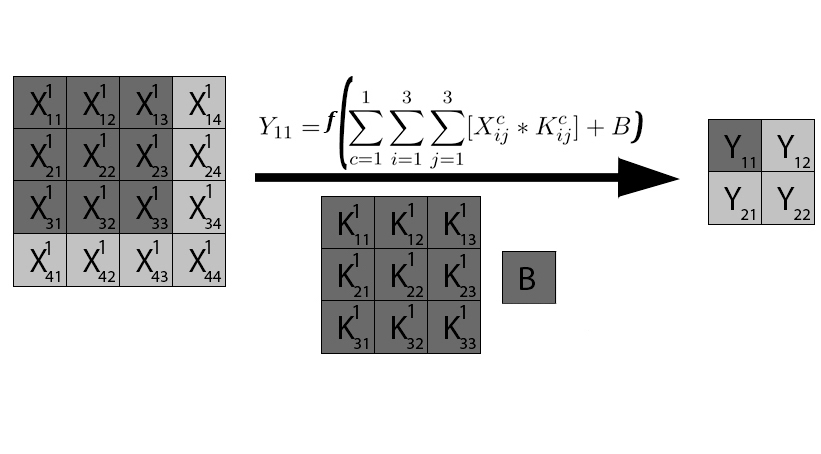
\includegraphics[width=1.2\linewidth]{imagenes/conv_1_1canal.jpg}  
		\caption{Cálculo $Y_{11}$ con entrada X \\ de 1 canal de profundidad}
	\end{subfigure}%
	\begin{subfigure}{.5\textwidth}
		\hspace{10mm}
		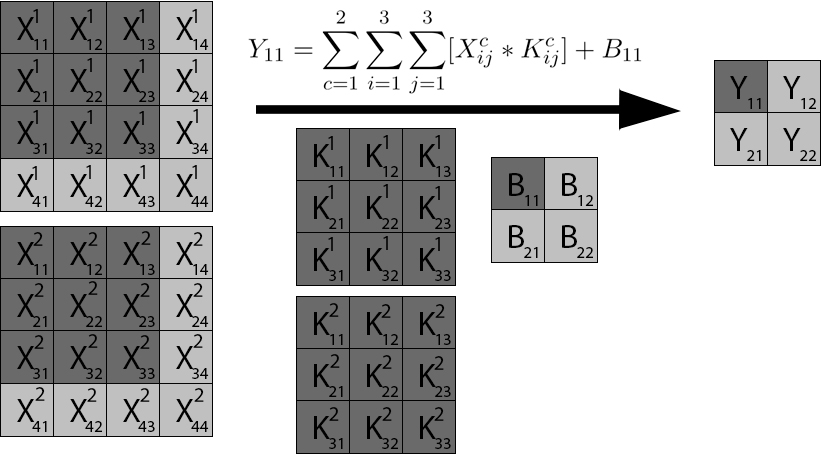
\includegraphics[width=1.2\linewidth]{imagenes/conv_1_2canales.jpg}  
		\caption{Cálculo $Y_{11}$ con entrada X \\ de 2 canales de profundidad}
	\end{subfigure}
	
	\vspace{5mm}
	\begin{subfigure}{.5\textwidth}
		\hspace{-10mm}
		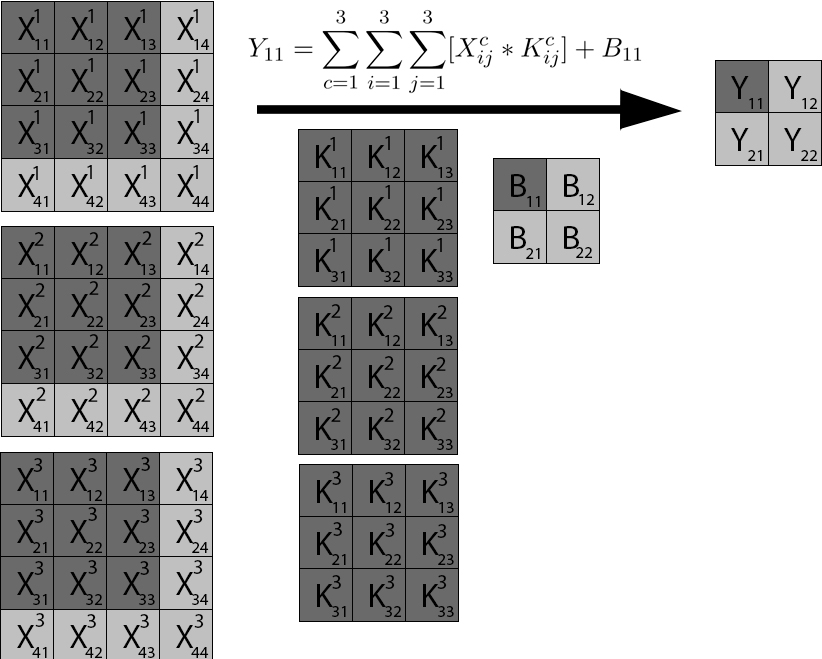
\includegraphics[width=1.2\linewidth]{imagenes/conv_1_3canales.jpg}  
		\caption{Cálculo $Y_{11}$ con entrada X \\ de 3 canales de profundidad}
	\end{subfigure}
	\caption{Propagación hacia delante en una capa convolucional con varios canales de profundidad}
	\label{fig:forward_prop_convolucional_canales_profundidad}
\end{figure}

De esta forma, en la Figura \ref{fig:forward_prop_convolucional_canales_profundidad} se muestra como una convolución con C canales de profundidad se descompone en la suma de C convoluciones con un canal de profundidad. \\ Para una entrada X con C canales de profundidad, convolución(X,K) = convolución($X^1,K^1$) + convolución($X^2,K^2$) + ... + convolución($X^C,K^C$). \\
Por último, en cada ``paso'' del ``deslizamiento'' se suma un solo sesgo y se aplica una sola vez la función de activación, independientemente del número de canales de profundidad que presente la entrada X.

\subsubsection{Propagación hacia delante, número de filtros}

\begin{figure}[H]
	\centering
	\begin{subfigure}{.5\textwidth}
		\hspace{-10mm}
		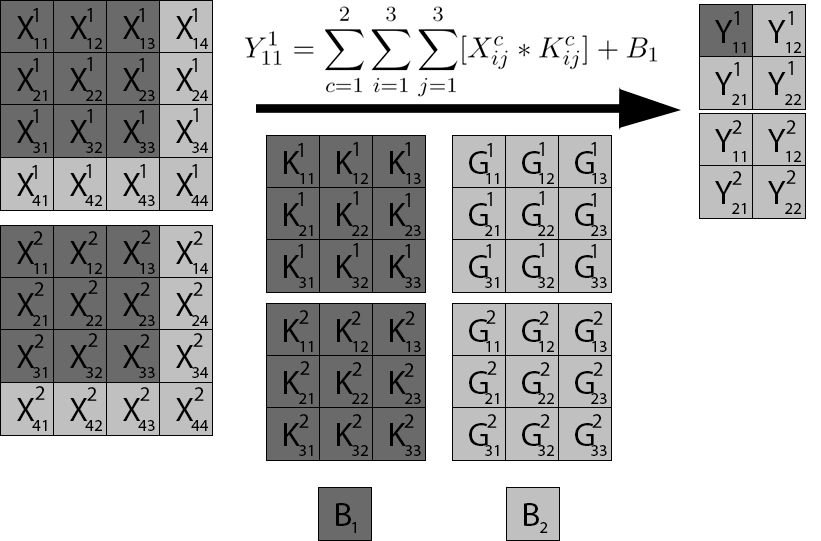
\includegraphics[width=1.2\linewidth]{imagenes/conv_2kernels_1.jpg}  
		\caption{Cálculo de $Y^1_{11}$ con el filtro K}
	\end{subfigure}%
	\begin{subfigure}{.5\textwidth}
		\hspace{10mm}
		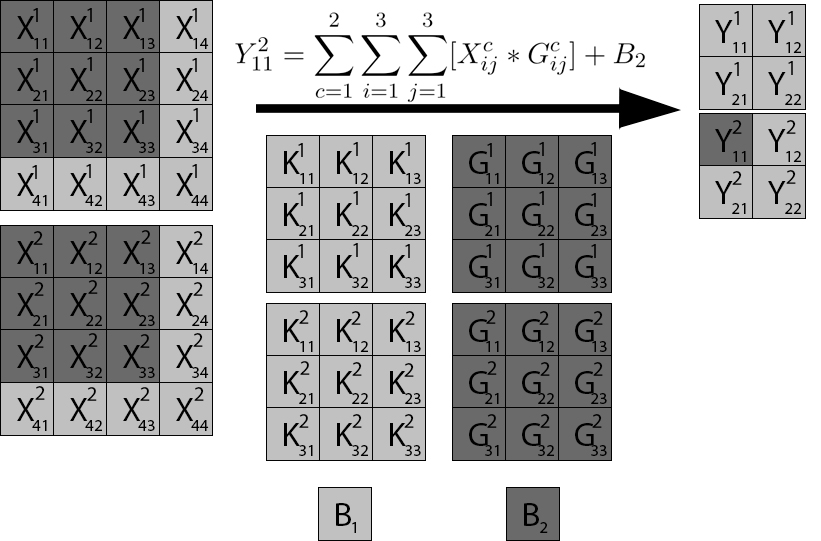
\includegraphics[width=1.2\linewidth]{imagenes/conv_2kernels_2.jpg}  
		\caption{Cálculo $Y^2_{11}$ con el filtro G}
	\end{subfigure}
	\caption{Propagación hacia delante en una capa convolucional con varios filtros}
	\label{fig:forward_prop_convolucional_varios_kernels}
\end{figure}

Cada convolución entre dos volúmenes 3D produce un volumen de salida 2D. Por tanto, al aplicar N convoluciones entre un volumen de entrada X y una serie de filtros K=$\{K_1, K_2, ..., K_N\}$, se obtendrá un volumen 3D de salida con tantas capas de profundidad como convoluciones se aplicaron (N). \\
En la Figura \ref{fig:forward_prop_convolucional_varios_kernels} se observa como al aplicar N=2 convoluciones sobre la misma entrada X (una con el filtro K y otra con el filtro G) se obtiene un volumen de salida con 2 capas de profundidad \cite{capa_convolucional_Stanford}.

\subsubsection{Relleno o ``Padding''}

En la figura \ref{fig:forward_prop_convolucional} se visualiza como al realizar una convolución entre un volumen X con dimensiones 1x4x4 y un kernel de pesos K con dimensiones 1x3x3, el resultado obtenido es un volumen Y de dimensiones 1x2x2. La reducción de dimensionalidad es un problema pues afecta directamente al número de convoluciones que se pueden aplicar sobre un volumen. \\
Por tanto, el ``relleno' o ``padding'' se aplica antes de realizar una convolución y es una técnica empleada para conservar las dimensiones espaciales de un volumen de entrada X, expandiendo cada canal del mismo tal y como se muestra en la figura \ref{fig:padding} \cite{padding_1}.

\begin{figure}[H]
	\centering
	\begin{subfigure}{.5\textwidth}
		\hspace{-15mm}
		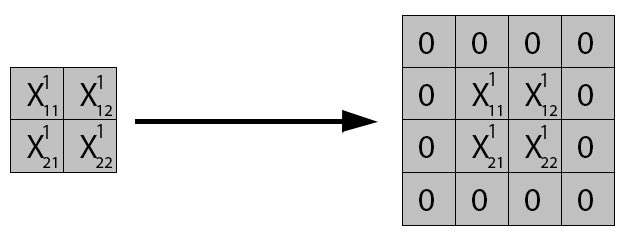
\includegraphics[width=1.2\linewidth]{imagenes/padding_a_1_nivel.jpg}  
		\caption{1 nivel de relleno}
	\end{subfigure}%
	\begin{subfigure}{.5\textwidth}
		\hspace{5mm}
		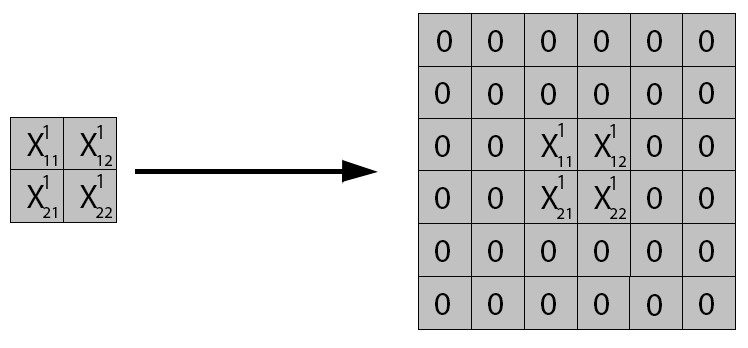
\includegraphics[width=1.2\linewidth]{imagenes/padding_a_2_niveles.jpg}  
		\caption{2 niveles de relleno}
	\end{subfigure}
	\caption{Relleno sobre un volumen de entrada X}
	\label{fig:padding}
\end{figure}

De esta forma, un relleno a un nivel sobre un volumen añadirá sobre el mismo dos filas y dos columnas con valores igual a 0. Un relleno a dos niveles añadirá cuatro filas y columnas con valores igual a cero, ..., un relleno a n niveles añadirá 2*n filas y columnas con valores igual a 0.

\subsubsection{Relleno completo}

Se denomina como relleno completo aquel que asegura que cada valor o casilla de X sea visitada el mismo número de veces que el resto \cite{padding_2}.

\begin{figure}[H]
	\centering
	\subfloat[1 nivel de relleno]{%
		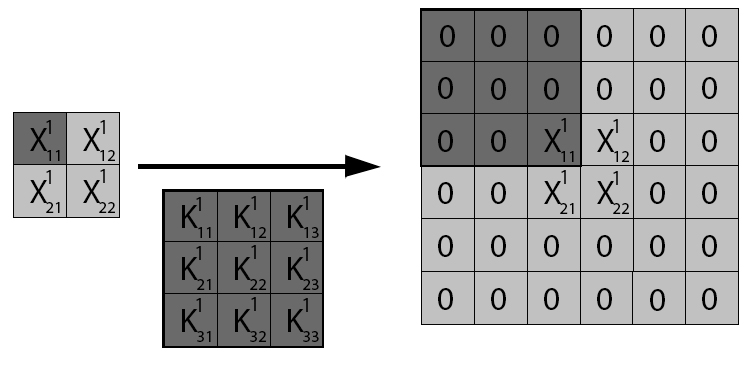
\includegraphics[width=0.45\textwidth]{imagenes/conv_padding_1.jpg}%
		\label{fig:sub1}%
	}\hfill
	\subfloat[2 niveles de relleno]{%
		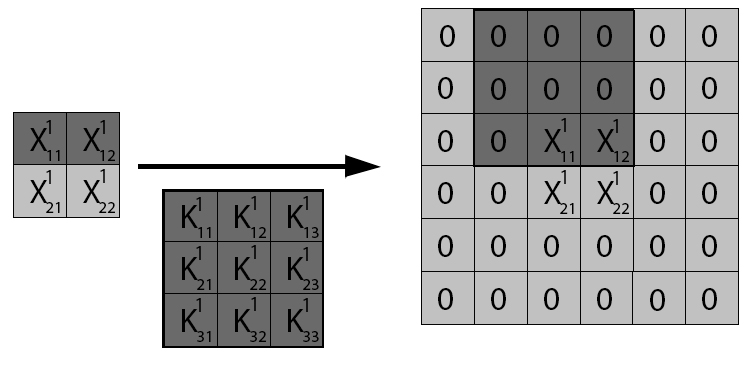
\includegraphics[width=0.45\textwidth]{imagenes/conv_padding_2.jpg}%
		\label{fig:sub2}%
	}\\
	\subfloat[1 nivel de relleno]{%
		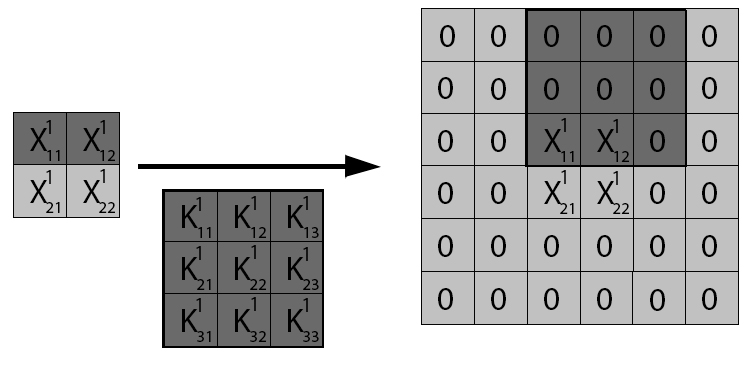
\includegraphics[width=0.45\textwidth]{imagenes/conv_padding_3.jpg}%
		\label{fig:sub3}%
	}\hfill
	\subfloat[2 niveles de relleno]{%
		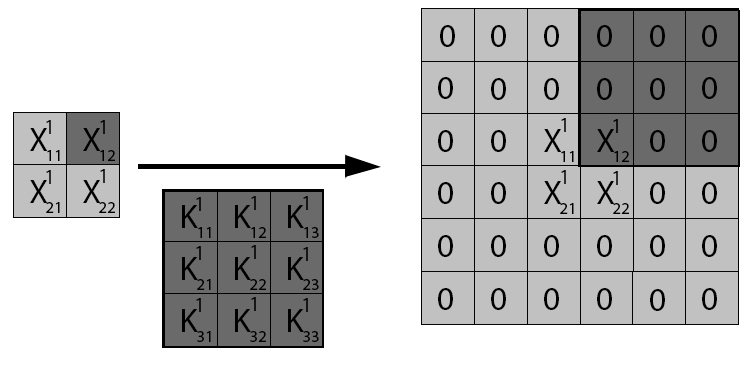
\includegraphics[width=0.45\textwidth]{imagenes/conv_padding_4.jpg}%
		\label{fig:sub4}%
	}\hfill
	
	\caption{Relleno sobre un volumen de entrada X}
\end{figure}

\begin{figure}[H]\ContinuedFloat
	\centering
	\subfloat[1 nivel de relleno]{%
		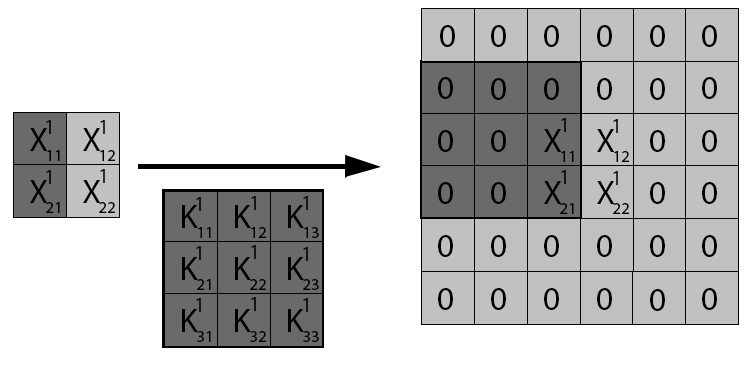
\includegraphics[width=0.45\textwidth]{imagenes/conv_padding_5.jpg}%
		\label{fig:sub5}%
	}\hfill
	\subfloat[2 niveles de relleno]{%
		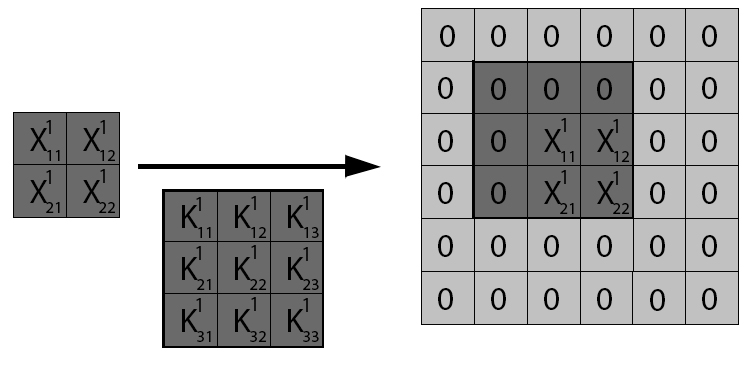
\includegraphics[width=0.45\textwidth]{imagenes/conv_padding_6.jpg}%
		\label{fig:sub6}%
	}\\
	\subfloat[1 nivel de relleno]{%
		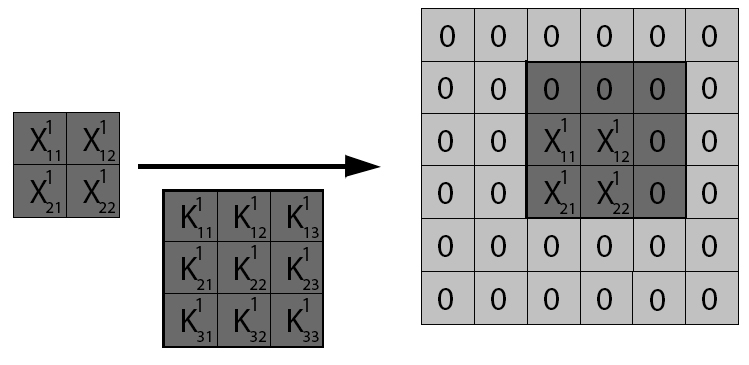
\includegraphics[width=0.45\textwidth]{imagenes/conv_padding_7.jpg}%
		\label{fig:sub7}%
	}\hfill
	\subfloat[2 niveles de relleno]{%
		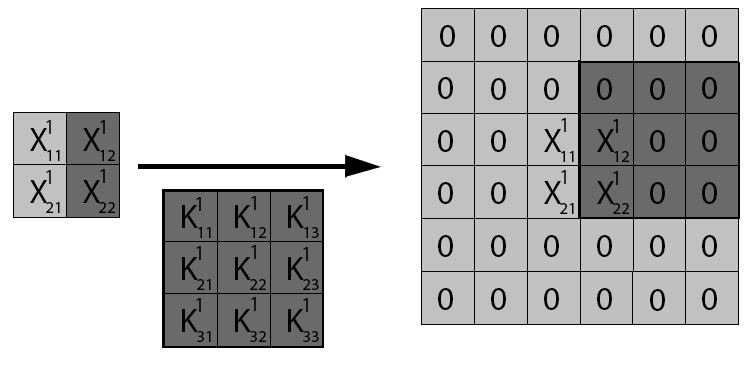
\includegraphics[width=0.45\textwidth]{imagenes/conv_padding_8.jpg}%
		\label{fig:sub8}%
	}\hfill
		\subfloat[1 nivel de relleno]{%
		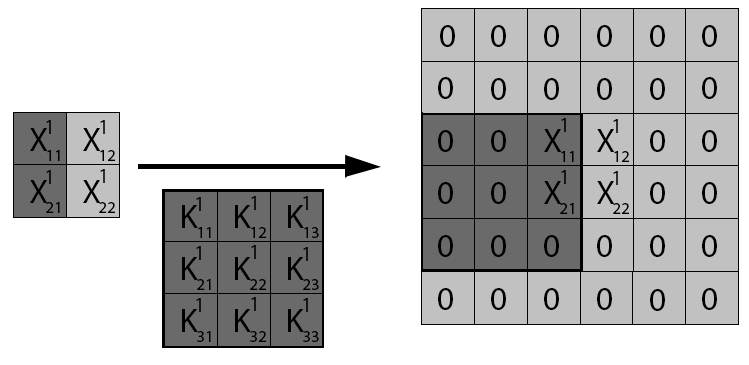
\includegraphics[width=0.45\textwidth]{imagenes/conv_padding_9.jpg}%
		\label{fig:sub9}%
	}\hfill
	\subfloat[2 niveles de relleno]{%
		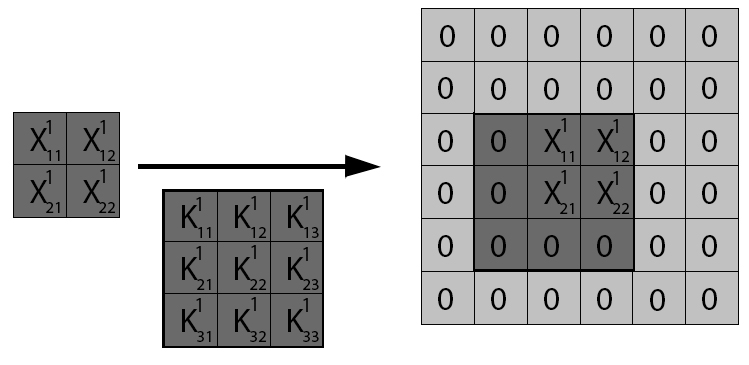
\includegraphics[width=0.45\textwidth]{imagenes/conv_padding_10.jpg}%
		\label{fig:sub10}%
	}\hfill
		\subfloat[1 nivel de relleno]{%
		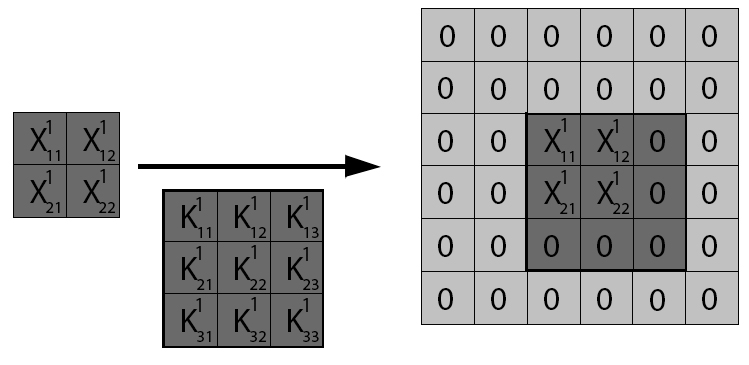
\includegraphics[width=0.45\textwidth]{imagenes/conv_padding_11.jpg}%
		\label{fig:sub11}%
	}\hfill
	\subfloat[2 niveles de relleno]{%
		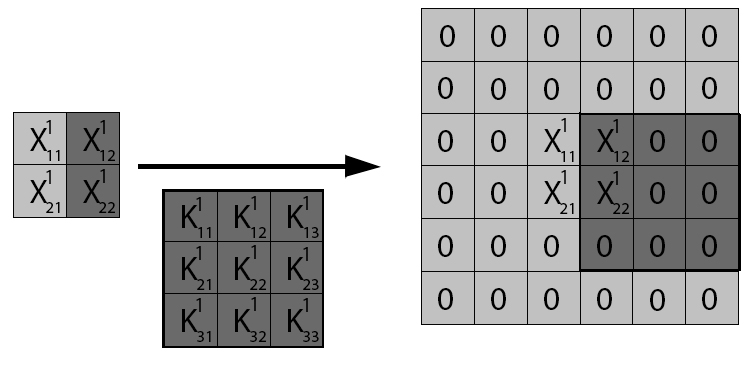
\includegraphics[width=0.45\textwidth]{imagenes/conv_padding_12.jpg}%
		\label{fig:sub12}%
	}\hfill
	\subfloat[1 nivel de relleno]{%
		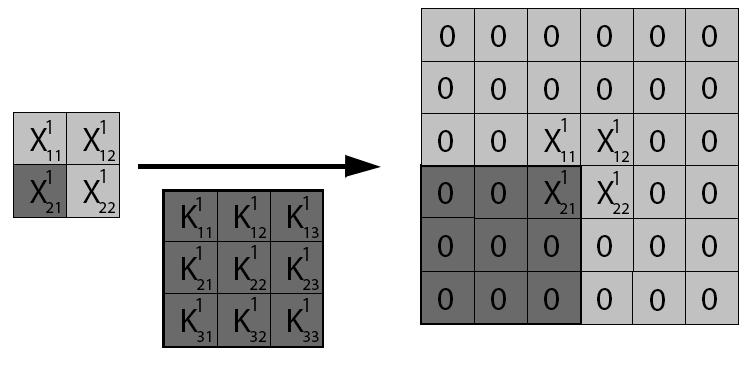
\includegraphics[width=0.45\textwidth]{imagenes/conv_padding_13.jpg}%
		\label{fig:sub13}%
	}\hfill
	\subfloat[2 niveles de relleno]{%
		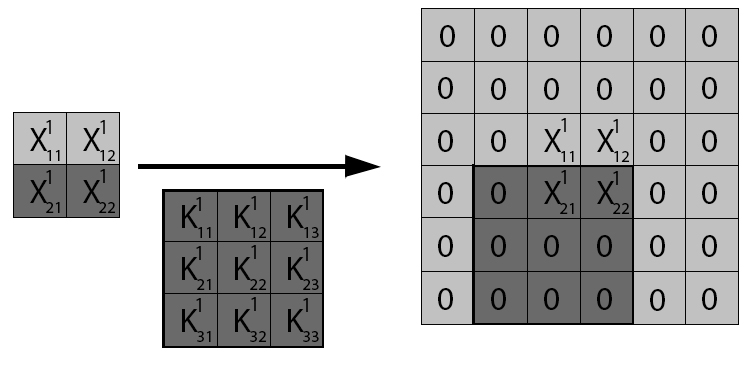
\includegraphics[width=0.45\textwidth]{imagenes/conv_padding_14.jpg}%
		\label{fig:sub14}%
	}\hfill
	\subfloat[1 nivel de relleno]{%
		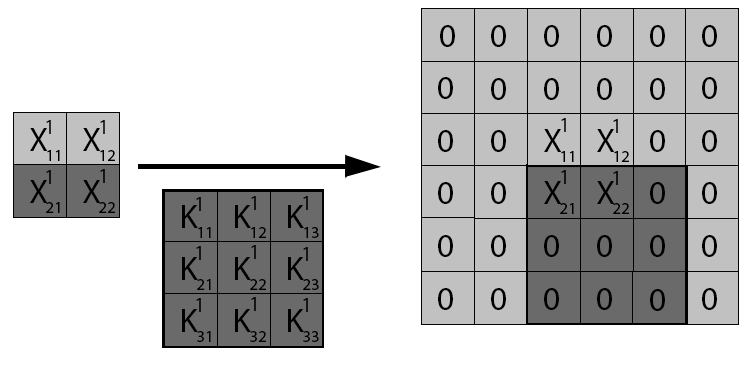
\includegraphics[width=0.45\textwidth]{imagenes/conv_padding_15.jpg}%
		\label{fig:sub15}%
	}\hfill
	\subfloat[2 niveles de relleno]{%
		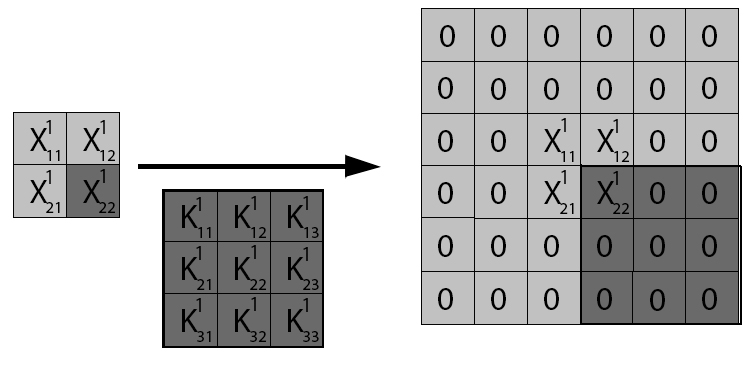
\includegraphics[width=0.45\textwidth]{imagenes/conv_padding_16.jpg}%
		\label{fig:sub16}%
	}\\
	
	\caption{Relleno sobre un volumen de entrada X}
	\label{fig:full_padding}
\end{figure}

Tal y como se muestra en la figura \ref{fig:full_padding}, se realiza un relleno completo pues en la convolución entre X y K se accede a cada valor de X el mismo número de veces (9).

\subsection{Capa de agrupación máxima}

\subsubsection{Componentes}

\begin{figure}[H]
	\centering
	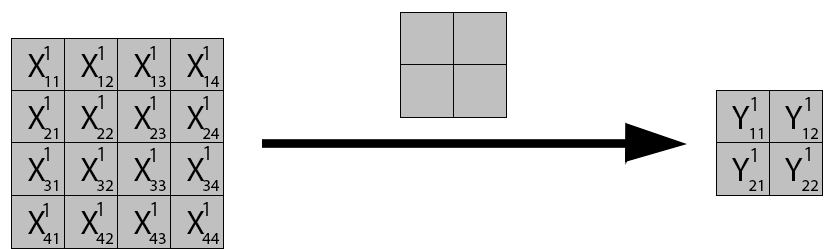
\includegraphics[scale=0.35]{imagenes/pool_nombres.jpg}  
	\caption{Componentes en una capa de agrupación máxima}
\end{figure}

Al igual que las capas convolucionales, las capas de agupación máxima también presentan una ``ventana'' que se irá deslizando por el volumen de entrada. Sin embargo, el resultado en cada iteración viene dado por el valor máximo contenido en ella. Por tanto, no presenta parámetros asociados.

\subsubsection{Propagación hacia delante}

\begin{figure}[H]
	\centering
	\begin{subfigure}{.5\textwidth}
		\hspace{-10mm}
		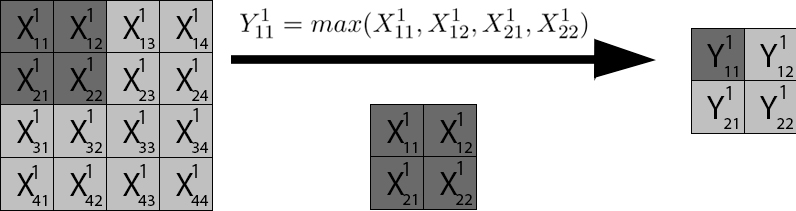
\includegraphics[width=1.2\linewidth]{imagenes/maxpool_1.jpg}  
		\caption{Cálculo $Y_{11}$}
	\end{subfigure}%
	\begin{subfigure}{.5\textwidth}
		\hspace{10mm}
		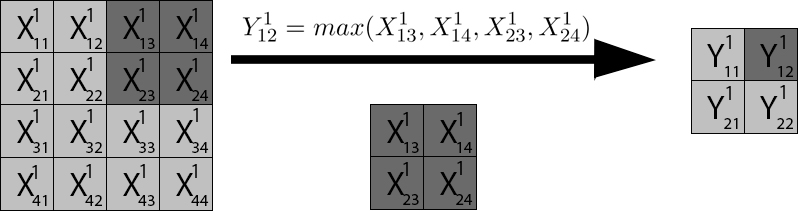
\includegraphics[width=1.2\linewidth]{imagenes/maxpool_2.jpg}  
		\caption{Cálculo $Y_{12}$}
	\end{subfigure}
	
	\vspace{5mm}
	\begin{subfigure}{.5\textwidth}
		\hspace{-10mm}
		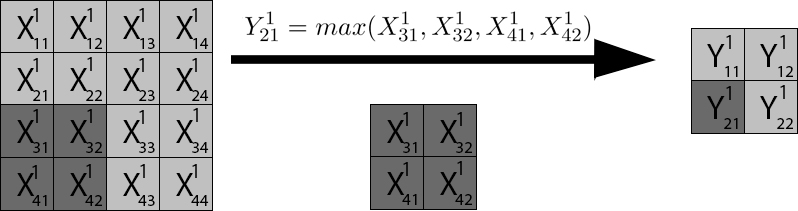
\includegraphics[width=1.2\linewidth]{imagenes/maxpool_3.jpg}  
		\caption{Cálculo $Y_{21}$}
	\end{subfigure}%
	\begin{subfigure}{.5\textwidth}
		\hspace{10mm}
		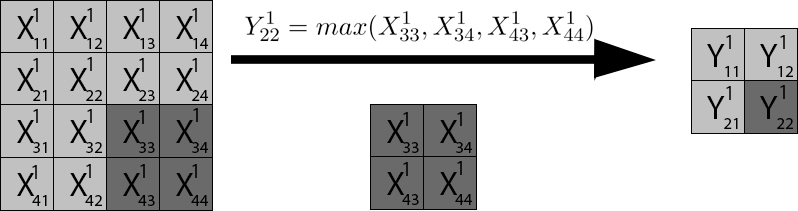
\includegraphics[width=1.2\linewidth]{imagenes/maxpool_4.jpg}  
		\caption{Cálculo $Y_{22}$}
	\end{subfigure}
	\caption{Propagación hacia delante en una capa de agrupación máxima}
	\label{fig:forward_prop_maxpool}
\end{figure}

A diferencia de las capas convolucionales, las capas de agrupación máxima no comparten regiones del volumen de entrada entre distintas iteraciones. Esto se muestra en las figuras \ref{fig:forward_prop_maxpool} y \ref{fig:forward_prop_convolucional}.


\subsubsection{Propagación hacia delante, canales de profundidad}

\begin{figure}[H]
	\centering
	\begin{subfigure}{.5\textwidth}
		\hspace{-10mm}
		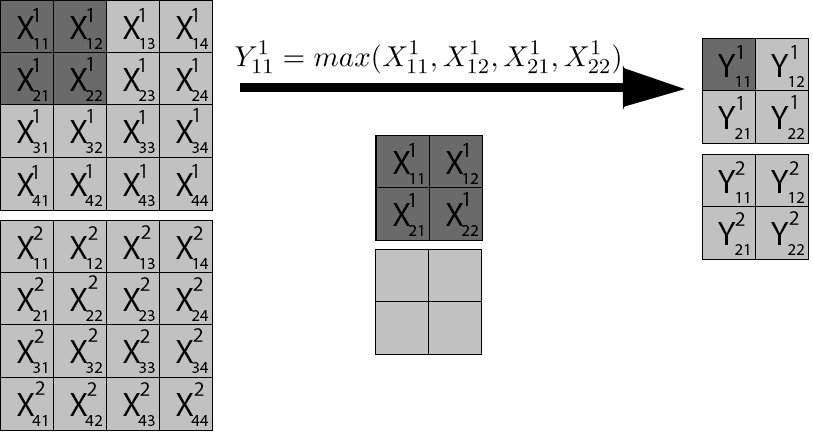
\includegraphics[width=1.2\linewidth]{imagenes/maxpool_2capas_1.jpg}  
		\caption{Cálculo $Y_{11}$}
	\end{subfigure}%
	\begin{subfigure}{.5\textwidth}
		\hspace{10mm}
		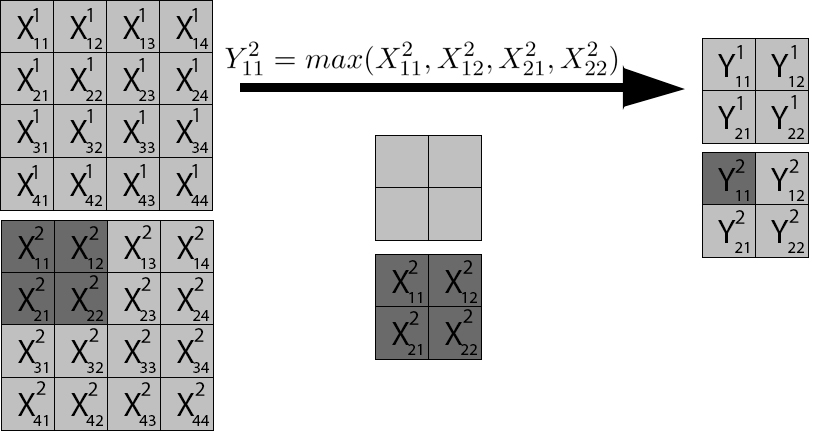
\includegraphics[width=1.2\linewidth]{imagenes/maxpool_2capas_2.jpg}  
		\caption{Cálculo $Y_{12}$}
	\end{subfigure}
	
	\caption{Propagación hacia delante en una capa de agrupación máxima}
	\label{fig:forward_prop_maxpool_canales_profundidad}
\end{figure}

Tal y como se muestra en la figura \ref{fig:forward_prop_maxpool_canales_profundidad}, cada ``ventana'' se desliza sobre el volumen de entrada en un canal de profundidad distinto.

\subsubsection{Propagación hacia detrás}

\begin{figure}[H]
	\centering
	\begin{subfigure}{.5\textwidth}
		\hspace{-10mm}
		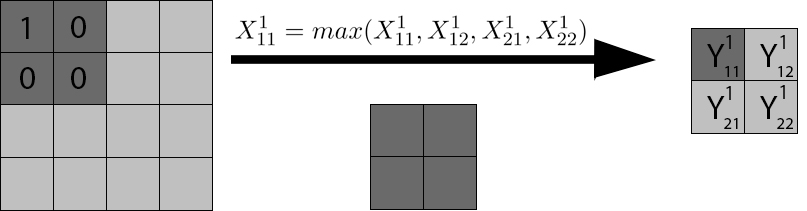
\includegraphics[width=1.2\linewidth]{imagenes/back_maxpool_1.jpg}  
		\caption{Cálculo $Y_{11}$}
	\end{subfigure}%
	\begin{subfigure}{.5\textwidth}
		\hspace{10mm}
		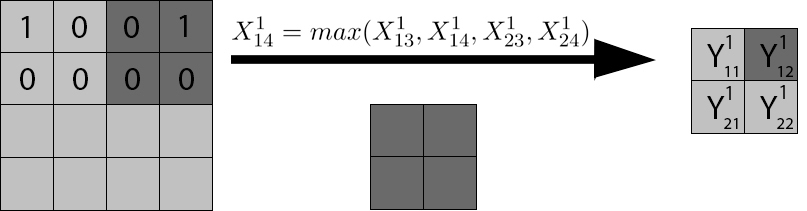
\includegraphics[width=1.2\linewidth]{imagenes/back_maxpool_2.jpg}  
		\caption{Cálculo $Y_{12}$}
	\end{subfigure}
	
	\begin{subfigure}{.5\textwidth}
		\hspace{-10mm}
		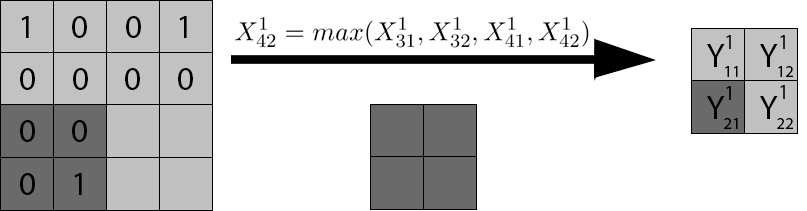
\includegraphics[width=1.2\linewidth]{imagenes/back_maxpool_3.jpg}  
		\caption{Cálculo $Y_{11}$}
	\end{subfigure}%
	\begin{subfigure}{.5\textwidth}
		\hspace{10mm}
		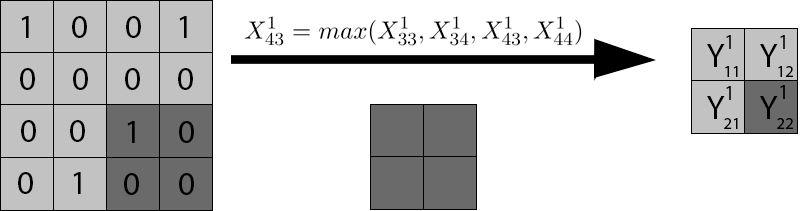
\includegraphics[width=1.2\linewidth]{imagenes/back_maxpool_4.jpg}  
		\caption{Cálculo $Y_{12}$}
	\end{subfigure}%
	\caption{Propagación hacia delante en una capa de agrupación máxima}
	\label{fig:back_prop_maxpool}
\end{figure}

Para la primera iteración de la figura \ref{fig:back_prop_maxpool}, en la propagación hacia detrás se calcula el gradiente respecto al volumen de entrada de la siguiente forma:

\begin{gather}
	\frac{\partial E}{\partial X^1_{11}} = \frac{\partial E}{\partial Y} * \frac{\partial Y}{\partial X^1_{11}} \\
	\frac{\partial E}{\partial X^1_{12}} = \frac{\partial E}{\partial Y} * \frac{\partial Y}{\partial X^1_{12}} \\
	\frac{\partial E}{\partial X^1_{21}} = \frac{\partial E}{\partial Y} * \frac{\partial Y}{\partial X^1_{21}} \\
	\frac{\partial E}{\partial X^1_{22}} = \frac{\partial E}{\partial Y} * \frac{\partial Y}{\partial X^1_{22}}
\end{gather}

 
Tomando el ejemplo de la figura \ref{fig:back_prop_maxpool} (a), se obtiene que $Y^1_{11} = X^1_{11}$. Por tanto, las fórmulas anteriores se convierten en:

\begin{gather}
	\frac{\partial E}{\partial X^1_{11}} = \frac{\partial E}{\partial Y} * \frac{\partial X^1_{11}}{\partial X^1_{11}} = \frac{\partial E}{\partial Y} * 1 = \frac{\partial E}{\partial Y} \\
	\frac{\partial E}{\partial X^1_{12}} = \frac{\partial E}{\partial Y} * \frac{\partial X^1_{11}}{\partial X^1_{12}} = \frac{\partial E}{\partial X^1_{11}} * 0 \\
	\frac{\partial E}{\partial X^1_{21}} = \frac{\partial E}{\partial Y} * \frac{\partial X^1_{11}}{\partial X^1_{21}} = \frac{\partial E}{\partial X^1_{11}} * 0 \\
	\frac{\partial E}{\partial X^1_{22}} = \frac{\partial E}{\partial Y} * \frac{\partial X^1_{11}}{\partial X^1_{22}} = \frac{\partial E}{\partial X^1_{11}} * 0
\end{gather}


 
Como el resultado obtenido en cada iteración solo depende del valor máximo de la ventana, tiene sentido que la derivada de la salida Y respecto a la entrada X sea igual a 1 solo en dicho caso y 0 en el resto \cite{max_pool_backprop} \cite{max_pool_backprop_2}.
\subsection{Capa de aplanado}

\subsubsection{Propagación hacia delante}
\begin{figure}[H]
	\centering
	\begin{subfigure}{.5\textwidth}
		\hspace{-10mm}
		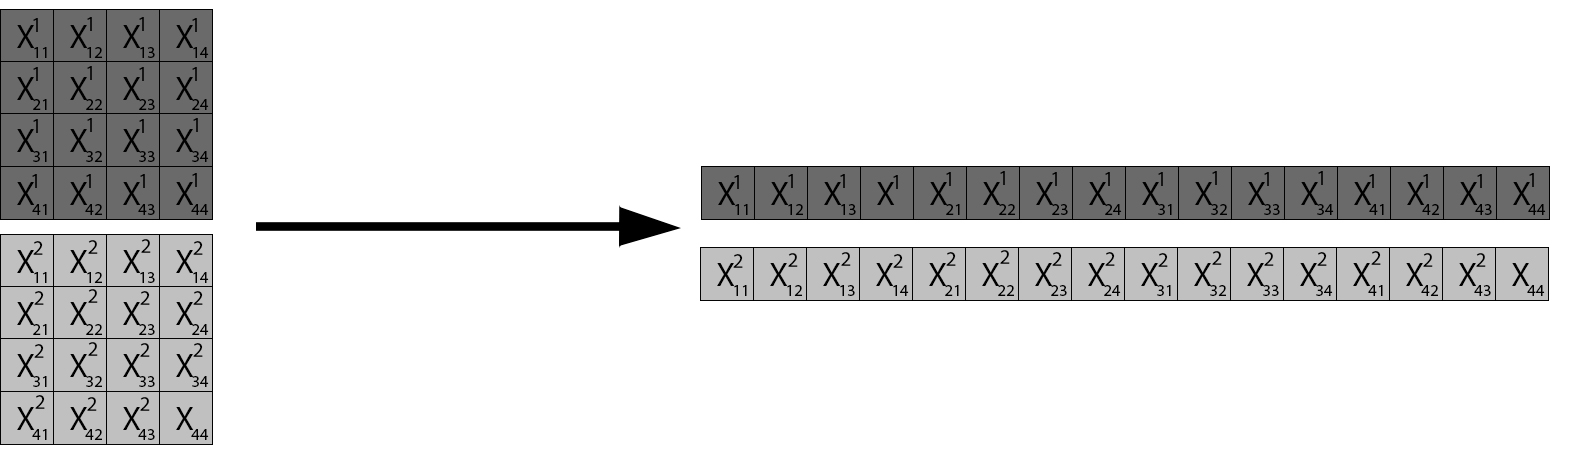
\includegraphics[width=2\linewidth]{imagenes/flatten_1.jpg}  
		\caption{Propagación hacia delante de la capa de aplanado con la primera capa de profundidad}
	\end{subfigure}
	\begin{subfigure}{.5\textwidth}
		\hspace{-10mm}
		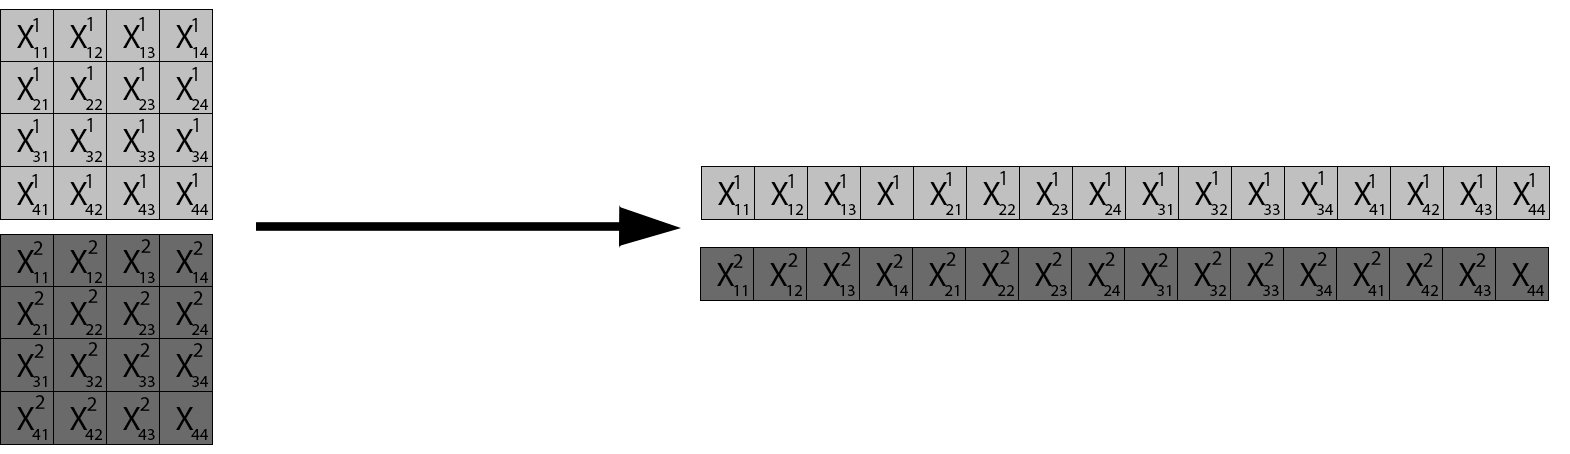
\includegraphics[width=2\linewidth]{imagenes/flatten_2.jpg}  
		\caption{Propagación hacia delante de la capa de aplanado con la segunda capa de profundidad}
	\end{subfigure}
	
	\caption{Propagación hacia delante en una capa de agrupación máxima}
	\label{fig:forward_prop_flatten_canales_profundidad}
\end{figure}

La capa de aplanado tiene como objetivo la creación de un ``enlace'' entre las capas de convolución y agrupación con la capas totalmente conectadas. En la propagación hacia delante, parte de un volumen de entrada 3D para, mediante un ``aplanado'', convertirlo en un vector 1D que pueda ser usado como entrada para una red totalmente conectada. \\
Como solo se modifica la forma en la que se agrupan los datos, no requiere la presencia de parámetros \cite{flatten_forward}.

\subsubsection{Propagación hacia detrás}

\begin{figure}[H]
	\centering
	\begin{subfigure}{.5\textwidth}
		\hspace{-30mm}
		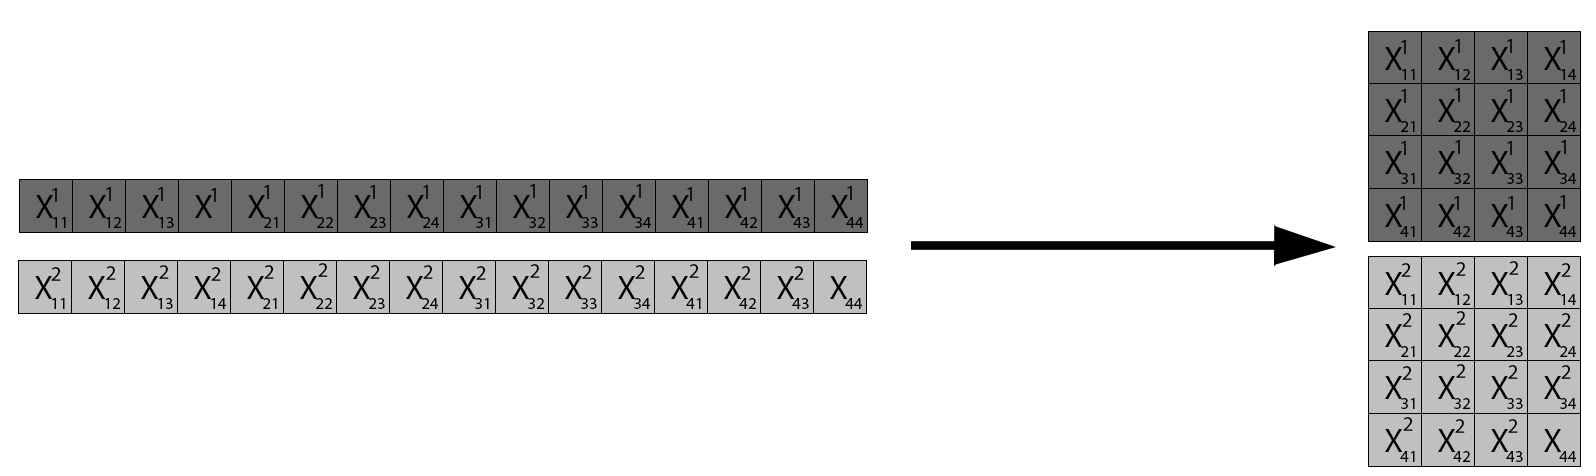
\includegraphics[width=2\linewidth]{imagenes/back_flatten_1.jpg}  
		\caption{Propagación hacia detrás de la capa de aplanado con la primera capa de profundidad}
	\end{subfigure}
	\begin{subfigure}{.5\textwidth}
		\hspace{-30mm}
		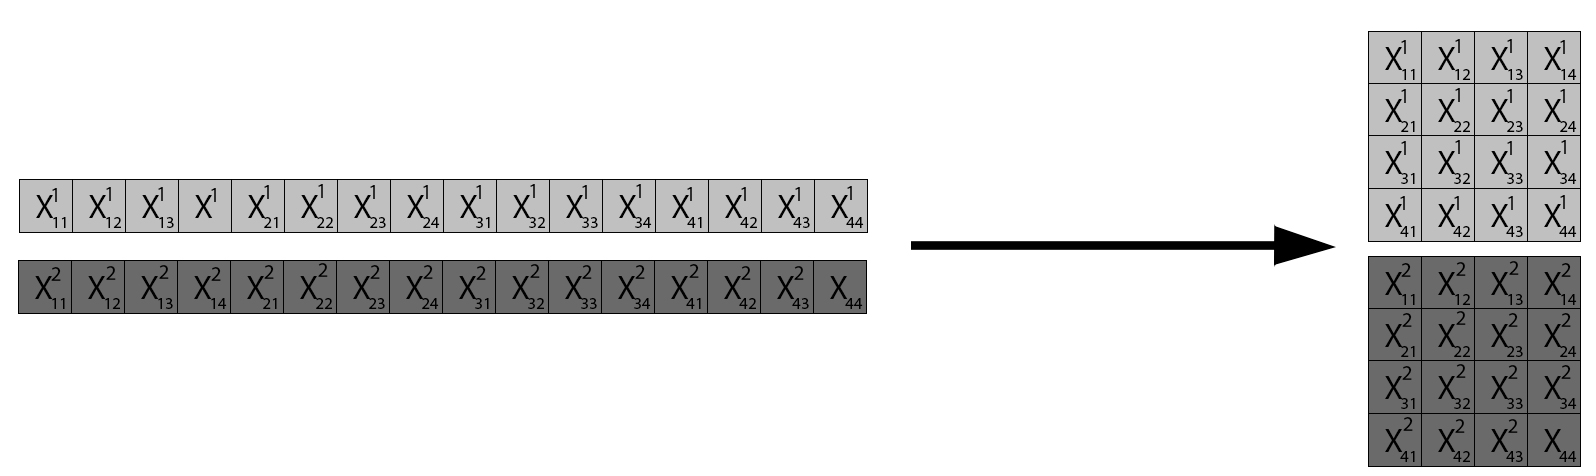
\includegraphics[width=2\linewidth]{imagenes/back_flatten_2.jpg}  
		\caption{Propagación hacia detrás de la capa de aplanado con la segunda capa de profundidad}
	\end{subfigure}
	
	\caption{Propagación hacia delante en una capa de agrupación máxima}
	\label{fig:back_prop_flatten_canales_profundidad}
\end{figure}

En la propagación hacia detrás, se parte de un array 1D y se convierte en un volumen 3D que pueda ser usado como entrada para una capa convolucional o de agrupación
\cite{flatten_forward}.

\section{cuDNN (Deep Neural Network)}

Es una librería de primitivas acelerada por GPU para redes neuronales profundas. Proporciona implementaciones altamente optimizadas para rutinas estándar como la propagación hacia delante y hacia detrás en capas convolucionales, de agrupación máxima, e incluso con funciones de activación como ReLU o sigmoide, entre otras \cite{cuDNN}. \\
Su meta es obtener el mejor rendimiento posible en GPUs de NVIDIA para casos importantes de aprendizaje profundo. Dados sus buenos resultados, se emplea en gran cantidad de frameworks de aprendizaje profundo, siendo algunos de ellos Caffe2, Keras, MATLAB, Pytorch, o TensorFlow \cite{cuDNN_librerias}. \\
Está diseñada para ser utilizada en aplicaciones de aprendizaje profundo que requieran un poder computacional intensivo, permitiendo a desarrolladores e investigadores aprovechar al máximo las prestaciones de las GPUs de NVIDIA. Entre ellas, destaca la compatibilidad con múltiples arquitecturas de  GPU, su optimización de la memoria, y su flexibilidad y facilidad de integración. Por todo esto y más, se ha convertido en un compotente esencial en el desarrollo de soluciones de inteligencia artificial, facilitando la investigación y la innovación en el campo del aprendizaje profundo.


\subsection{Manejador}

cuDNN asume que los datos necesarios se encuentran ya en GPU y accesibles desde device. Se hablará de esto con más detalle en la sección sobre cuda y GPU. \\
Una aplicación que use cuDNN requiere de la inicialización de un manejador o handle. Dicho manejador será requerido por cuDNN en cada operación que se quiera realizar con dicha librería, permitiendo al usuario un control explícito sobre el funcionamiento de la misma aunque este emplee múltiples hebras o GPUs. \\
Por ejemplo, en el caso de múltiples GPUs, se pueden asociar diferentes dispositivos con diferentes hebras del host, de forma que cada una tenga un manejador de cuDNN distinto. Así, las llamadas a cuDNN con distinto manejador se ejecutarán en distinta GPU \cite{cuDNN_core_concepts}.

\subsection{Tensores}

Las operaciones en cuDNN reciben tensores como entrada y producen tensores como salida \cite{cuDNN_core_concepts}.

\subsubsection{Tensor 3D}
Un tensor 3D se suele emplear para representar un volumen 3D como podría ser una imagen RGB. Sus dimensiones se describen mediante 3 letras: B, M y N.

\begin{enumerate}
	\item \textbf{B}: Tamaño del batch
	\item \textbf{M}: Filas por imagen 2D
	\item \textbf{N}: Columnas por imagen 2D
\end{enumerate}

\subsubsection{Tensor 4D}
Suele representar conjuntos de imágenes 2D. Sus dimensiones son N, C, H, W

\begin{enumerate}
	\item \textbf{N}: Tamaño del batch
	\item \textbf{C}: Número de imágenes 2D
	\item \textbf{H}: Filas por imagen 2D
	\item \textbf{W}: Columnas por imagen 2D
\end{enumerate}

cuDNN permite varios formatos pero usaremos NCHW por compatibilidad con el resto de implementaciones desarrolladas en este proyecto.


\subsubsection{Representación de un tensor 4D}

\begin{figure}[H]
	\centering
	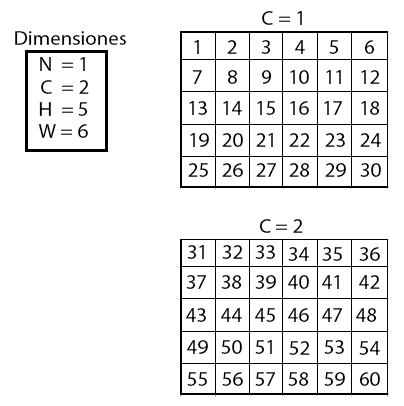
\includegraphics[scale=0.5]{imagenes/ejemplo_tensor.png}  
	\caption{Ejemplo de tensor 4D con dimensiones: N=1, C=1, H=5, y W=6}
	\label{fig:ejemplo_tensor}
\end{figure}

En la figura \ref{fig:ejemplo_tensor} se muestra un conjunto de imágenes 3D con las siguientes dimensiones:
\begin{enumerate}
	\item \textbf{N}: Tamaño del batch, 1
	\item \textbf{C}: Número de imágenes 2D o canales por imagen 3D, 2
	\item \textbf{H}: Filas por imagen 2D, 5
	\item \textbf{W}: Columnas por imagen 2D, 6
\end{enumerate}

\begin{figure}[H]
	\centering
	\includegraphics[scale=0.5]{imagenes/tensor_nchw.png}  
	\caption{Ejemplo de tensor 4D NCHW con dimensiones: N=1, C=1, H=5, y W=6}
	\label{fig:tensor_nchw}
\end{figure}

En la figura \ref{fig:tensor_nchw} se muestra como se almacena en memoria el volumen de datos de la figura \ref{fig:ejemplo_tensor} según el formato NCHW. Esto es, por cada imagen 3D n$\in$\{0,...,N\}, almacenar cada canal c$\in$\{0,...,C\} según una ordenación por filas.

\subsection{Principales funciones}

A continuación se mencionarán las principales funciones de cuDNN que se han empleado en este proyecto, siendo las responsables tanto de la propagación hacia delante como de la retropropagación en capas convolucionales y de agrupación máxima, entre otras.

\subsubsection{cudnnConvolutionForward}
Realiza la propagación hacia delante en una capa convolucional.

\begin{verbatim}
	cudnnStatus_t cudnnConvolutionForward(
	cudnnHandle_t                       handle,
	const void                         *alpha,
	const cudnnTensorDescriptor_t       xDesc,
	const void                         *x,
	const cudnnFilterDescriptor_t       wDesc,
	const void                         *w,
	const cudnnConvolutionDescriptor_t  convDesc,
	cudnnConvolutionFwdAlgo_t           algo,
	void                               *workSpace,
	size_t                              workSpaceSizeInBytes,
	const void                         *beta,
	const cudnnTensorDescriptor_t       yDesc,
	void                               *y)
\end{verbatim}

\begin{enumerate}
	\item \textbf{handle}: Manejador.
	\item \textbf{alpha, beta}: Punteros a escalares empleados para combinar los resultados con valores anteriores tal que valor\_final = alpha*result + beta*valor\_anterior.
	\item \textbf{xDesc}: Descriptor asociado al tensor de entrada.
	\item \textbf{x}: Puntero a los datos de entrada en GPU asociados con el descriptor de tensor xDesc.
	\item \textbf{wDesc}: Descriptor asociado al tensor de pesos.
	\item \textbf{w}: Puntero a los pesos en GPU asociados con el descriptor de tensor wDesc.
	\item \textbf{convDesc}: Descriptor de convolución.
	\item \textbf{algo}: Especifica qué algoritmo de convolución aplicar.
	\item \textbf{workSpace}: Puntero a un espacio de trabajo en memoria de GPU.
	\item \textbf{workSpaceSizeInBytes}: Especifica el tamaño en bytes de workSpace.
	\item \textbf{yDesc}: Descriptor asociado al tensor de salida.
	\item \textbf{y}: Puntero a los datos de salida en GPU asociados con el descriptor de tensor yDesc.
\end{enumerate}
\cite{cuDNN_conv_fwd}

\subsubsection{cudnnPoolingForward}
Se encarga de la propagación hacia delante en una capa de agrupación máxima.

\begin{verbatim}
	cudnnStatus_t cudnnPoolingForward(
	cudnnHandle_t                    handle,
	const cudnnPoolingDescriptor_t   poolingDesc,
	const void                      *alpha,
	const cudnnTensorDescriptor_t    xDesc,
	const void                      *x,
	const void                      *beta,
	const cudnnTensorDescriptor_t    yDesc,
	void                            *y)
\end{verbatim}

\begin{enumerate}
	\item \textbf{handle}: Manejador.
	\item \textbf{poolingDesc}: Descriptor de la operación de agrupación.
	\item \textbf{alpha, beta}: Punteros a escalares empleados para combinar los resultados con valores anteriores tal que valor\_final = alpha*result + beta*valor\_anterior.
	\item \textbf{xDesc}: Descriptor asociado al tensor de entrada.
	\item \textbf{x}: Puntero a los datos de entrada en GPU asociados con el descriptor de tensor xDesc.
	\item \textbf{yDesc}: Descriptor asociado al tensor de salida.
	\item \textbf{y}: Puntero a los datos de salida en GPU asociados con el descriptor de tensor yDesc.
\end{enumerate}
\cite{cuDNN_pool_fwd}

\subsubsection{cudnnPoolingBackward}
Realiza la retropropagación en una capa de agrupación máxima.

\begin{verbatim}
	cudnnStatus_t cudnnPoolingBackward(
	cudnnHandle_t                       handle,
	const cudnnPoolingDescriptor_t      poolingDesc,
	const void                         *alpha,
	const cudnnTensorDescriptor_t       yDesc,
	const void                         *y,
	const cudnnTensorDescriptor_t       dyDesc,
	const void                         *dy,
	const cudnnTensorDescriptor_t       xDesc,
	const void                         *xData,
	const void                         *beta,
	const cudnnTensorDescriptor_t       dxDesc,
	void                               *dx)
\end{verbatim}

\begin{enumerate}
	\item \textbf{handle}: Manejador.
	\item \textbf{poolingDesc}: Descriptor de la operación de agrupación.
	\item \textbf{alpha, beta}: Punteros a escalares empleados para combinar los resultados con valores anteriores tal que valor\_final = alpha*result + beta*valor\_anterior.
	\item \textbf{yDesc}: Descriptor asociado al tensor de salida.
	\item \textbf{y}: Puntero a los datos de salida en GPU asociados con el descriptor de tensor yDesc.
	\item \textbf{dyDesc}: Descriptor asociado al tensor que almacena el gradiente de la pérdida respecto a los datos de salida.
	\item \textbf{dy}: Puntero al gradiente de la pérdida respecto a los datos de salida en GPU asociados con el descriptor de tensor dyDesc.
	\item \textbf{xDesc}: Descriptor asociado al tensor de entrada.
	\item \textbf{x}: Puntero a los datos de entrada en GPU asociados con el descriptor de tensor xDesc.
	\item \textbf{dxDesc}: Descriptor asociado al tensor que almacena el gradiente de la pérdida respecto a los datos de entrada.
	\item \textbf{dx}: Puntero al gradiente de la pérdida respecto a los datos de entrada en GPU asociados con el descriptor de tensor dxDesc.	
\end{enumerate}
\cite{cuDNN_pool_fwd}

\subsubsection{cudnnConvolutionBackwardFilter}
Realiza la retropropagación respecto a los pesos en una capa convolucional.

\begin{verbatim}
	cudnnStatus_t cudnnConvolutionBackwardFilter(
	cudnnHandle_t                       handle,
	const void                         *alpha,
	const cudnnTensorDescriptor_t       xDesc,
	const void                         *x,
	const cudnnTensorDescriptor_t       dyDesc,
	const void                         *dy,
	const cudnnConvolutionDescriptor_t  convDesc,
	cudnnConvolutionBwdFilterAlgo_t     algo,
	void                               *workSpace,
	size_t                              workSpaceSizeInBytes,
	const void                         *beta,
	const cudnnFilterDescriptor_t       dwDesc,
	void                               *dw)
\end{verbatim}

\begin{enumerate}
	\item \textbf{handle}: Manejador.
	\item \textbf{alpha, beta}: Punteros a escalares empleados para combinar los resultados con valores anteriores tal que valor\_final = alpha*result + beta*valor\_anterior.
	\item \textbf{xDesc}: Descriptor asociado al tensor de entrada.
	\item \textbf{x}: Puntero a los datos de entrada en GPU asociados con el descriptor de tensor xDesc.	
	\item \textbf{dyDesc}: Descriptor asociado al tensor que almacena el gradiente de la pérdida respecto a los datos de salida.
	\item \textbf{dy}: Puntero al gradiente de la pérdida respecto a los datos de salida en GPU asociados con el descriptor de tensor dyDesc.
	\item \textbf{convDesc}: Descriptor de convolución.
	\item \textbf{algo}: Especifica qué algoritmo de convolución aplicar.
	\item \textbf{workSpace}: Puntero a un espacio de trabajo en memoria de GPU.
	\item \textbf{workSpaceSizeInBytes}: Especifica el tamaño en bytes de workSpace.
	\item \textbf{dwDesc}: Descriptor del tensor asociado al gradiente de la pérdida respecto a los pesos.
	\item \textbf{dw}: Puntero al gradiente de los pesos en GPU asociados con el descriptor de tensor dwDesc.
\end{enumerate}
\cite{cuDNN_conv_back_w}


\subsubsection{cudnnConvolutionBackwardData}
Realiza la retropropagación respecto a los datos de entrada en una capa convolucional.

\begin{verbatim}
	cudnnStatus_t cudnnConvolutionBackwardData(
	cudnnHandle_t                       handle,
	const void                         *alpha,
	const cudnnFilterDescriptor_t       wDesc,
	const void                         *w,
	const cudnnTensorDescriptor_t       dyDesc,
	const void                         *dy,
	const cudnnConvolutionDescriptor_t  convDesc,
	cudnnConvolutionBwdDataAlgo_t       algo,
	void                               *workSpace,
	size_t                              workSpaceSizeInBytes,
	const void                         *beta,
	const cudnnTensorDescriptor_t       dxDesc,
	void                               *dx)
\end{verbatim}

\begin{enumerate}
	\item \textbf{handle}: Manejador.
	\item \textbf{alpha, beta}: Punteros a escalares empleados para combinar los resultados con valores anteriores tal que valor\_final = alpha*result + beta*valor\_anterior.
	\item \textbf{wDesc}: Descriptor asociado al tensor de pesos.
	\item \textbf{w}: Puntero a los pesos en GPU asociados con el descriptor de tensor wDesc.
	\item \textbf{dyDesc}: Descriptor asociado al tensor que almacena el gradiente de la pérdida respecto a los datos de salida.
	\item \textbf{dy}: Puntero al gradiente de la pérdida respecto a los datos de salida en GPU asociados con el descriptor de tensor dyDesc.
	\item \textbf{convDesc}: Descriptor de convolución.
	\item \textbf{algo}: Especifica qué algoritmo de convolución aplicar.
	\item \textbf{workSpace}: Puntero a un espacio de trabajo en memoria de GPU.
	\item \textbf{workSpaceSizeInBytes}: Especifica el tamaño en bytes de workSpace.
	\item \textbf{dxDesc}: Descriptor asociado al tensor que almacena el gradiente de la pérdida respecto a los datos de entrada.
	\item \textbf{dx}: Puntero al gradiente de la pérdida respecto a los datos de entrada en GPU asociados con el descriptor de tensor dxDesc.	
\end{enumerate}
\cite{cuDNN_conv_back_x}
